% % % % % % % % % % % % % % % % % % % % % % % % % % % % % % % % % % % % % % % % 
% 
% Mensch-Maschine-Kommunikation 1 (ab WS 2016/17)
% Formelsammlung von LaTeX4EI
%
% @encode: 	UTF-8, tabwidth = 4, newline = LF
% @author:	Lukas Kompatscher
% @date:	18.03.2016
%
% % % % % % % % % % % % % % % % % % % % % % % % % % % % % % % % % % % % % % % % 


% Dokumenteinstellungen
% ======================================================================

% Dokumentklasse (Schriftgröße 6, DIN A4, Latex4EI Sheet)
\documentclass[german,color,6pt]{latex4ei/latex4ei_sheet}

% Just for testing, comment out!
%\usepackage{showframe}

% Additional Packages
\usepackage{multirow}
\usepackage{makecell}

% Additional Definitions and Formats
\graphicspath{{img/}} 
\definecolor{darkgreen}{rgb}{0,0.5,0}
\DeclareTextFontCommand{\emph}{\bfseries}
\makeatletter
\renewcommand\paragraph{\@startsection{paragraph}{4}{\z@}%
	{3.25ex \@plus1ex \@minus.2ex}%
	{-1em}%
	{\normalfont\normalsize\bfseries}}
\makeatother
\titlespacing{\paragraph}{0pt}{-10pt}{.5em}[]


% LaTeX4EI Definitions

\title{Mensch-Maschine-Kommunikation 1 \\ {\large (ab WS 2016/17)}}
\author{Lukas Kompatscher, Fabian Göttel und Hendrik Böttcher}
\myemail{lukas.kompatscher@tum.de}	

% Dokumentbeginn
% ======================================================================
\begin{document}

% TITLE ================================================================
\maketitle
%=======================================================================

% Die Unterteilung der Themen stimmt nicht exakt mit der Unterteilung der Vorlesung überein.

% SECTION 1: ALLGEMEINE EINFÜHRUNG =====================================
\section{Allgemeine Einführung}
% ======================================================================
\begin{sectionbox}
	\subsection{Grundbegriffe der MMK}
	\begin{tablebox}{p{0.2\textwidth}p{0.75\textwidth}}
		\emph{Interaktion} & Kommunikation zwischen Mensch und Maschine. \\
		\emph{Interaktives System} & System, das auf Eingaben reagiert und gegebenenfalls auch Ausgaben generiert. \\
		\emph{HCI} & Human-Computer Interaction. \\
		\emph{MMI} & Mensch-Maschine-Interface. \\
		\emph{Usability} & Gebrauchstauglichkeit bzw. Eignung eines Produkts. \\
		\emph{Usability Engineering} & Gestaltung und Testen eines Produktes mit dem Ziel optimaler Bedienbarkeit durch die Mensch-Maschine-Schnittstelle. \\
		\emph{Software-Ergonomie} & Wissenschaft über die Gestaltung von Programmen mit benutzerfreundlicher Mensch-Maschine-Schnittstelle. \\
		\emph{Medium} & Datenträger für Information, z.B. Papier oder CD. \\
		\emph{Multimedia} & Datenverarbeitung und -darstellung unter Nutzung verschiedener Medien, z.B. Text, Grafik und Audio und Video. \\
		\emph{Modalität} & Ein-/Ausgabekanal der menschlichen Kommunikation und Sinneswahrnehmung, z.B. Sprache, Zeigen, Gestik, Tastatur. \\
	\end{tablebox}
\end{sectionbox}

\begin{sectionbox}
	\subsection{Wichtigste Disziplinen der MMK}
	\begin{center}
		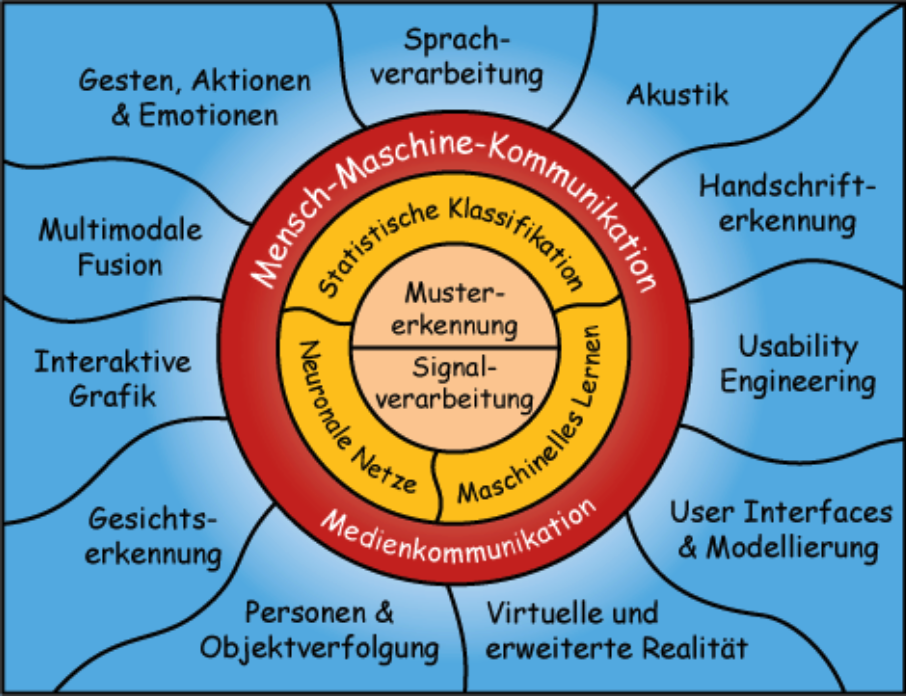
\includegraphics[width=0.9\textwidth]{mmk_diziplinen}
	\end{center}
\end{sectionbox}
\begin{sectionbox}
	\subsection{Trends in der MMK}
	\begin{itemize}
		\item Steigerung der Leistungsfähigkeit
		\item Reduzierung der Kosten
		\item Erweiterung der Funktionalität
		\item Verbesserung der Bedienbarkeit
	\end{itemize}
\end{sectionbox}

\begin{sectionbox}
	\subsection{Übersicht über Sinnesmodalitäten}
	\begin{tablebox}{lll}
		\emph{Sinnesbezeichnung}  & \emph{Modalität}   & \emph{Bemerkung}      \\ \cmrule
		Sehen                     & visuell            & \multirow{5}{*}{„5 Sinne“}             \\
		Hören                     & auditiv            & ~                     \\
		Riechen                   & olfaktorisch       & ~                     \\
		Schmecken                 & gustatorisch       & ~                     \\
		Tasten                    & taktil             & ~                     \\ \cmrule
		Druck                     & \multirow{2}{*}{haptisch}           & \multirow{2}{*}{mechanische Modal.} \\
		Kraft                     & ~                  & ~                     \\ \cmrule
		Berührung                 & \multirow{2}{*}{taktil}             & \multirow{2}{*}{oberflächen-sensitiv}  \\
		Vibration                 & ~                  & ~                     \\ \cmrule
		Temperatur                & thermorezeptorisch & ~                     \\ \cmrule
		Bewegung und Orientierung & kinästhetisch      & ~                     \\
		Gleichgewicht             & vestibulär         & ~                     \\
	\end{tablebox}
\end{sectionbox}

\begin{sectionbox}
	\subsection{Die Sinne des Menschen und ihre Datenraten}
	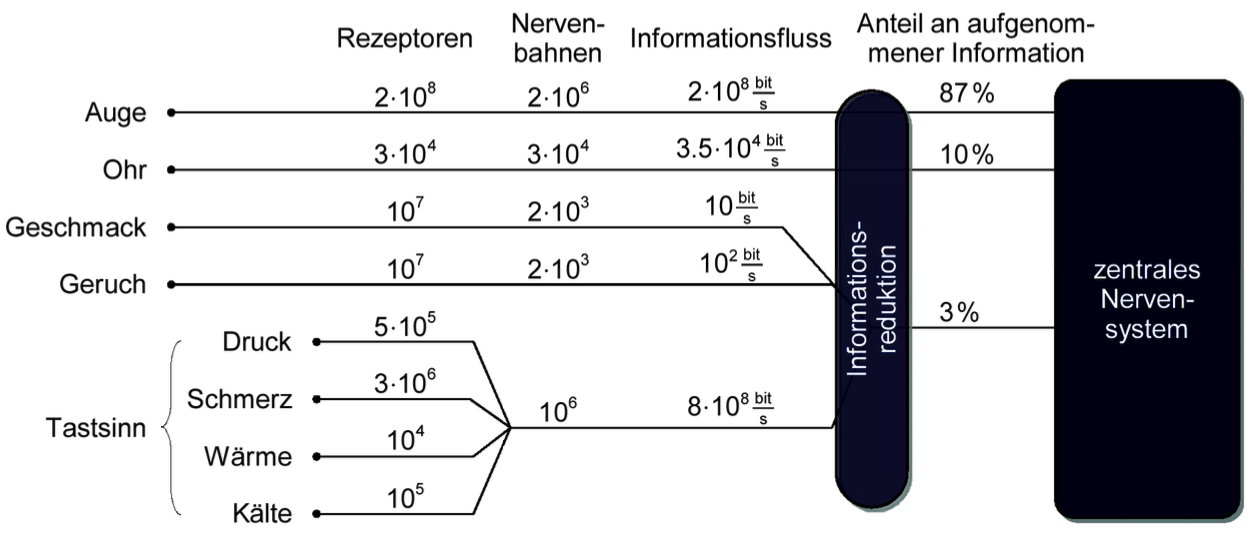
\includegraphics[width=\textwidth]{datenrate_sinne}
\end{sectionbox}

\begin{sectionbox}
	\subsection{Datenraten gängiger System der MMK}
	\begin{tablebox}{lll}
		System & Verhalten & Rate (KByte/sec) \\ \cmrule
		Tastatur (ungeübt) & Eingabe & 0.01 \\
		Tastatur (geübt) & Eingabe & 0.025 \\
		Handschrift & Eingabe & 0.0025 \\
		Spracheingabe & Eingabe & 0.01-0.02 \\
		Maus & Eingabe & 0.02 \\
		Sprachausgabe & Ausgabe & 0.6 \\
		Text lesen & Ausgabe & 0.03-0.3 \\
		Hören (CD) & Ausgabe & 40 \\
		Sehen (Video) & Ausgabe & 20000
	\end{tablebox}
\end{sectionbox}


% SECTION 2: SPRACHKOMMUNIKATION ======================================
\section{Sprachkommunikation}
% ======================================================================
\begin{symbolbox}
	Ermittlung der geäußerten Wortfolge aus einem vorliegenden Sprachsignal und Verarbeitung dieser Information. Die Sprachkommunikation hat größtes Potential aller Eingabemethoden, da sie auch beim Menschen die häufigste und natürlichste Kommunikationsform ist.
\end{symbolbox}

\begin{sectionbox}
	\subsection{Physikalische Wellen}
	\parbox{0.5\textwidth}{\emph{Transversalwelle:}}
	\parbox{0.45\textwidth}{\emph{Longitudinalwelle (z.B. Schall):}} \\
	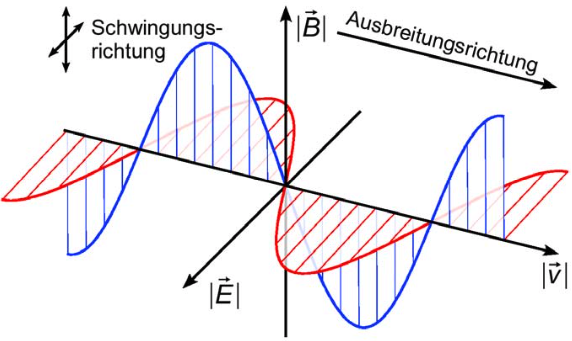
\includegraphics[width=0.45\textwidth]{transversalwelle}
	\hspace{0.05\textwidth}
	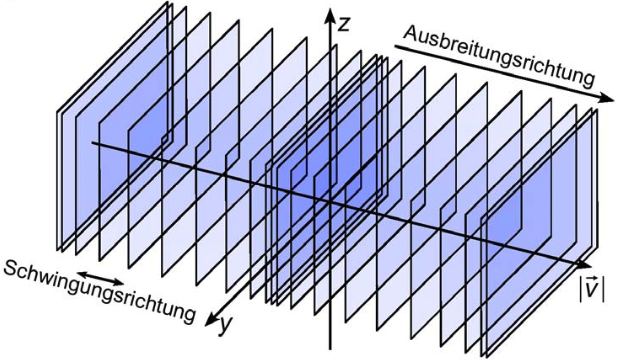
\includegraphics[width=0.45\textwidth]{longitudinalwelle}
\end{sectionbox}

\begin{sectionbox}
	\subsection{Schallquellen und ihre typischen Pegel}
	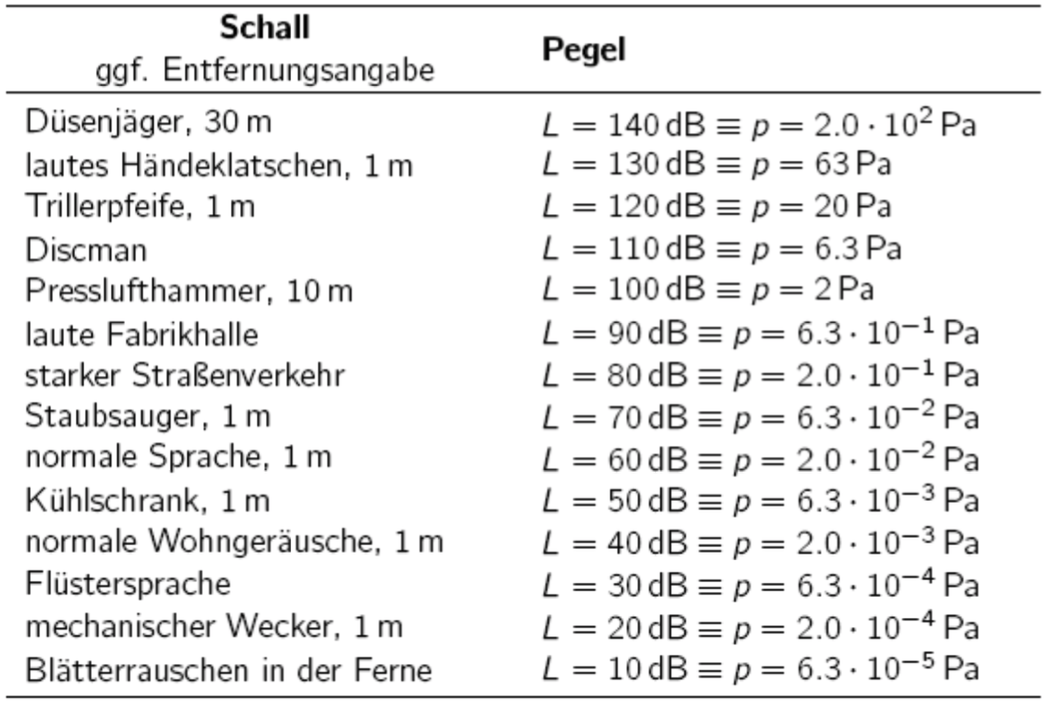
\includegraphics[width=\textwidth]{schallpegel}
\end{sectionbox}

\begin{sectionbox}
\subsection{Menschliche Hörsinn}
\subsubsection{Das Ohr}
	\paragraph{Außenohr} Ohrmuschel \& Gehörgang.\vspace{-1em}
	\paragraph{Mittelohr} Trommelfell, Gehörknöchelchen (Hammer, Amboss, Steigbügel) \& Euchstachische Röhre; Wandlung von Luftschwingung in mech. Schwingung.\vspace{-1em}
	\paragraph{Innenohr} Steigbügel über ovale Fenster in mit Flüssigkeit gefüllte Schnecke; Impedanzwandlung von Luft zu Flüssigkeit.\vspace{-1em}
	\paragraph{Basilarmembran} Haarzellen (25k - 30k Rezeptoren) wandeln Schwingung in elektronische Nervenimpulse Frequenz-Ort-Wandlung, Zerlegung in Frequenzanteile $\Ra$ Hörnerv (30k Nervenfasern) $\Ra$ Hirn
	\begin{center}
		\includegraphics[width=\textwidth]{ohr}
		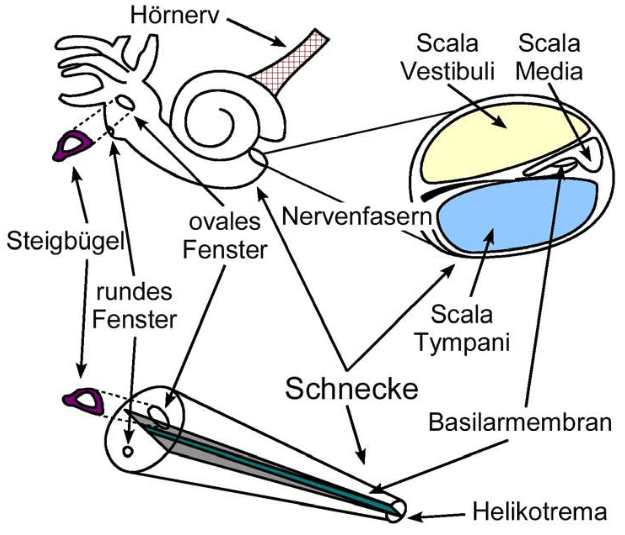
\includegraphics[width=0.7\textwidth]{ohr_detail}
	\end{center}
\end{sectionbox}

\begin{sectionbox}
	\subsubsection{Psychoakustik}
	\begin{itemize}
		\item Empfindlich von etwa 20 Hz - 20 kHz ($\approx$ 10 Oktaven)
		\item Starke Dämpfung für sehr niedrige und sehr hohe Frequenzen
		\item Resonanzfrequenz des Gehörgangs bei ca. $3 \dots 3.4 kHz$; 
		\item Lauteinheit in [sone] 1 sone $\triangleq$ Lautheit eines 1kHz Sinus mit 40 dB
		\item Verhältnistonhöhe [mel] 1000 mel $\triangleq$ 1000Hz
	\end{itemize}
	\begin{tablebox}{llll}
		\multicolumn{2}{c}{\emph{Psychoakustik}} &\multicolumn{2}{c}{\emph{Physik}}\\
		Bezeichnung & Einheit & Bezeichnung & Einheit\\
		\cmrule
		Tonheit $Z$ &Bark& \multirow{2}{*}{ Frequenz $f$ }& \multirow{2}{*}{$Hz$}\\
		Verhältnistonh. $V$ & Mel & & \\
		& & Schalldruck $p$ & $\frac{N}{m^2} = Pa$\\
		& & Schallschnelle $v$ & $\frac{m}{s}$\\
		& & Schallintensität $I$ & $\frac{W}{m^2} = \frac{N}{s m}$\\
		Lautstrk.pegel $L_n$ & Phon & \multirow{2}{*}{Schalldruckp. $L$} &\multirow{2}{*}{ $dB$}\\
		Lautheit $N$ & sone\\
		& & Schallleist. $P_{ak}$ & $W = \frac{N m}{s}$\\
		\cmrule
		\multicolumn{4}{c}{Bezugsschalldruck $p_0 = 2 \cdot 10^{-5} \frac{N}{m^2} = 20 \mu Pa$}\\
		\multicolumn{4}{c}{Bezugsintensität $I_0 = 1.0 \cdot 10^{-12} \frac{W}{m^2}$}\\
	\end{tablebox}
% \end{sectionbox}
% 
% \begin{sectionbox}
\vspace{-1em}\paragraph{Hörfläche} Jener Frequenz- und Pegelbereich von Schall, der vom menschlichen Gehör wahrgenommen werden kann:
\begin{center}
	\includegraphics[width=0.7\textwidth]{hoerflaeche}
	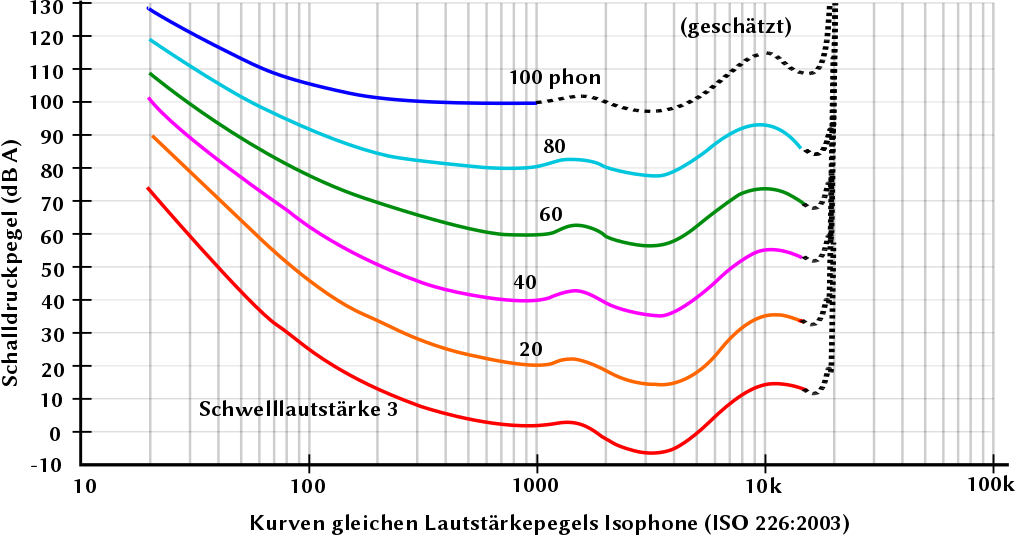
\includegraphics[width=\textwidth]{kurve_gleicher_lautstaerke}	
\end{center}

\vspace{-1em}\paragraph{Frequenzbewertung} Verfahren zur frequenzabhängigen Anpassung von Schalldruckpegeln an das menschliche Hörempfinden (nichtlinear zur Lautstärke). Hierfür werden verschiedene Filterkurven verwendet: A(20–40 phon), B(50–70 phon), C(80–90 phon), D(sehr hohe Schalldrücke) mit gleichem Lautstärkeeindruck. Lautheit $N$ in Sone ist angepasstes Schema.
\vspace{-1em}\paragraph{Frequenzgruppen} (24) begrenzte Auflösung des Gehörs; jede Frequenzgruppe nimmt gleiche Länge auf Basilarmembran ein (1,3mm - unter 500 Hz = 100Hz, drüber kleine Terz 1,19 der Mittenfrequenz); Bark-Skala; 1.31 Bark = 131 mel = 131 Hz.; Blätterrauschen in Ferne L = 10dB, Düsenjäger in 30 m L = 140dB.
\vspace{-1em}\paragraph{Verdeckungen} Hörschwelle bei Störschall (Maskierer); 
\begin{itemize}
	\item Spektrale: verbreitet sich mit steigendem Pegel überproportional.
	\item Zeitliche: Vorverdeckung; Simultanverdeckung; Nachverdeckung (einige hundert ms).
\end{itemize}
Kompression: Mithörschwelle über Verdeckungen ermitteln; MP3 ab 160 kBit/s.
\end{sectionbox}

\begin{sectionbox}
	\subsection{Menschliche Spracherzeugung}
	\begin{center}
		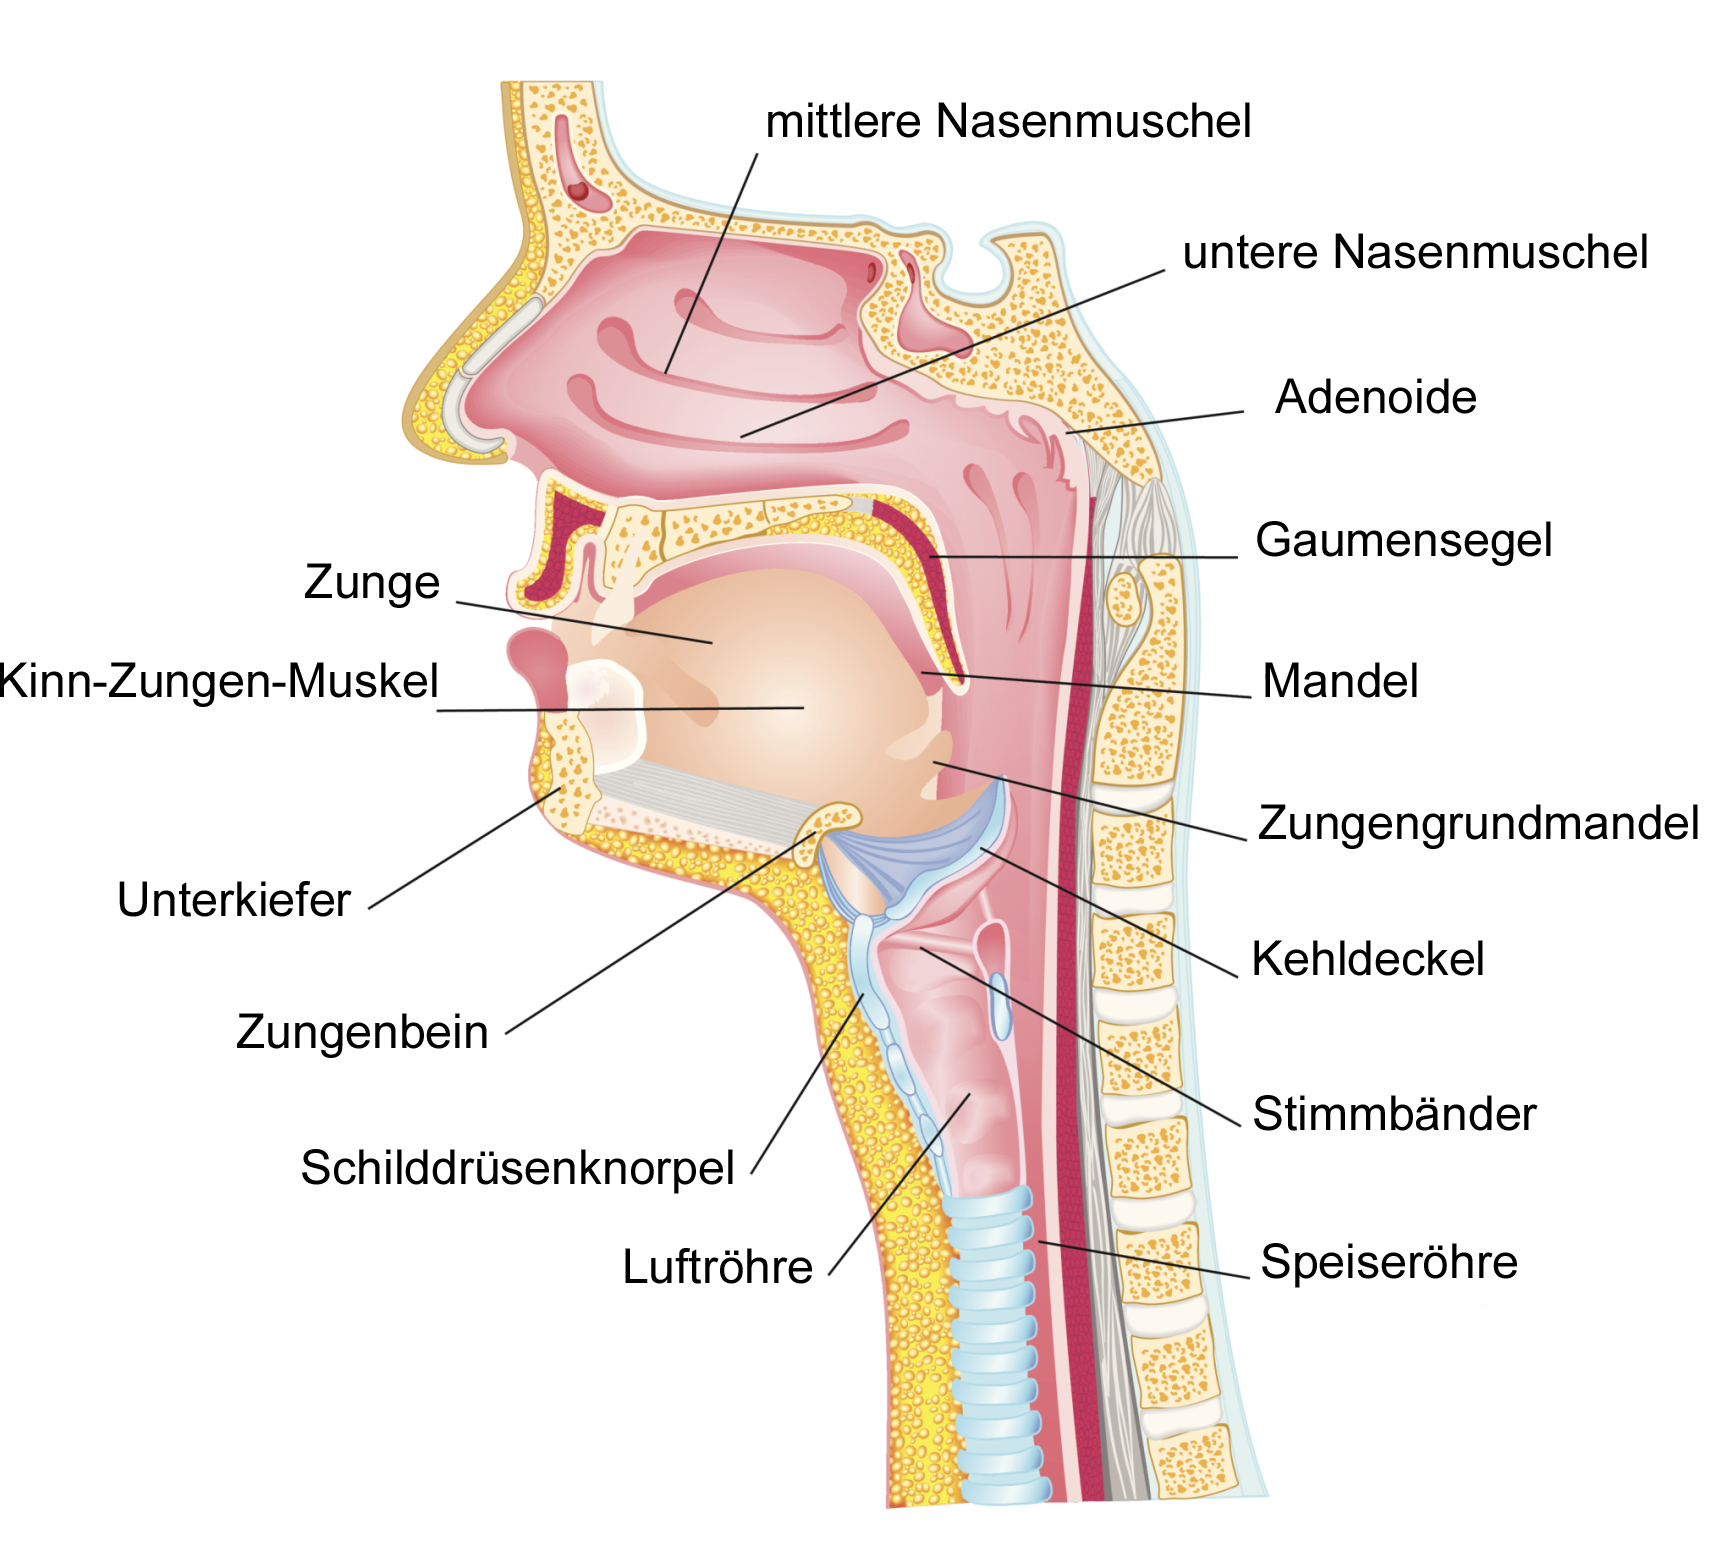
\includegraphics[width=0.8\textwidth]{hals_anatomie}	
	\end{center}
	\subsubsection{Phoneme}
	Das Phonem ist die kleinste bedeutungsunterscheidende Einheit des gesprochenen Wortes. \\ 
	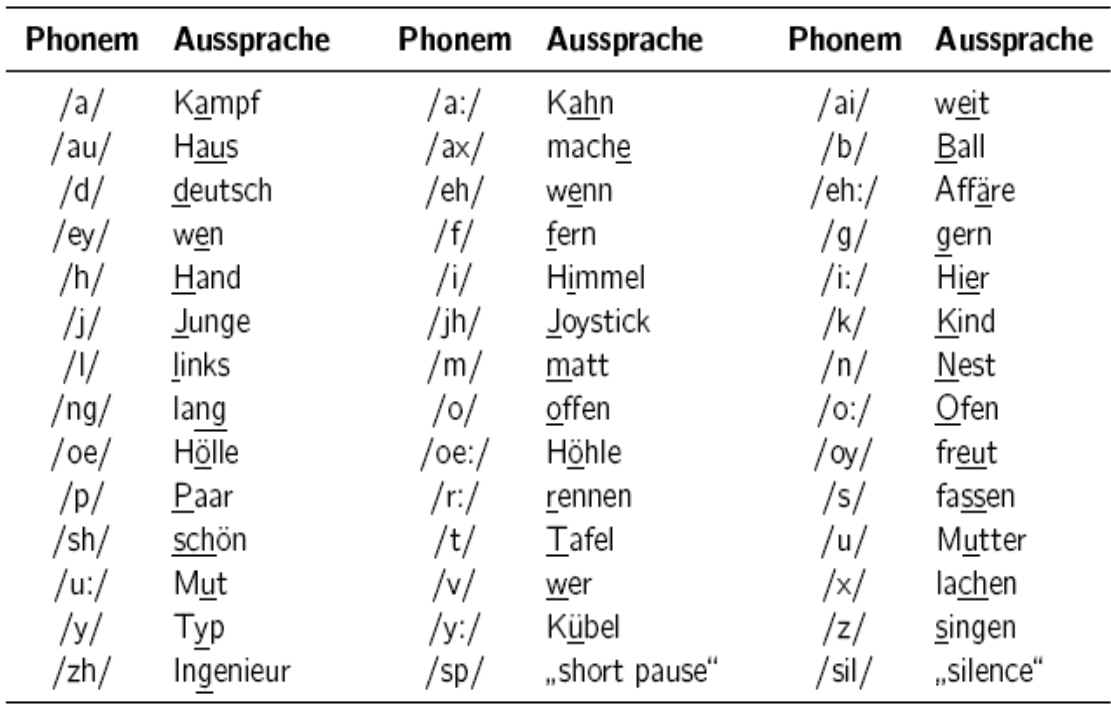
\includegraphics[width=\textwidth]{phoneme} \\
	Systematische Einteilung der Phoneme:
	\begin{center}
		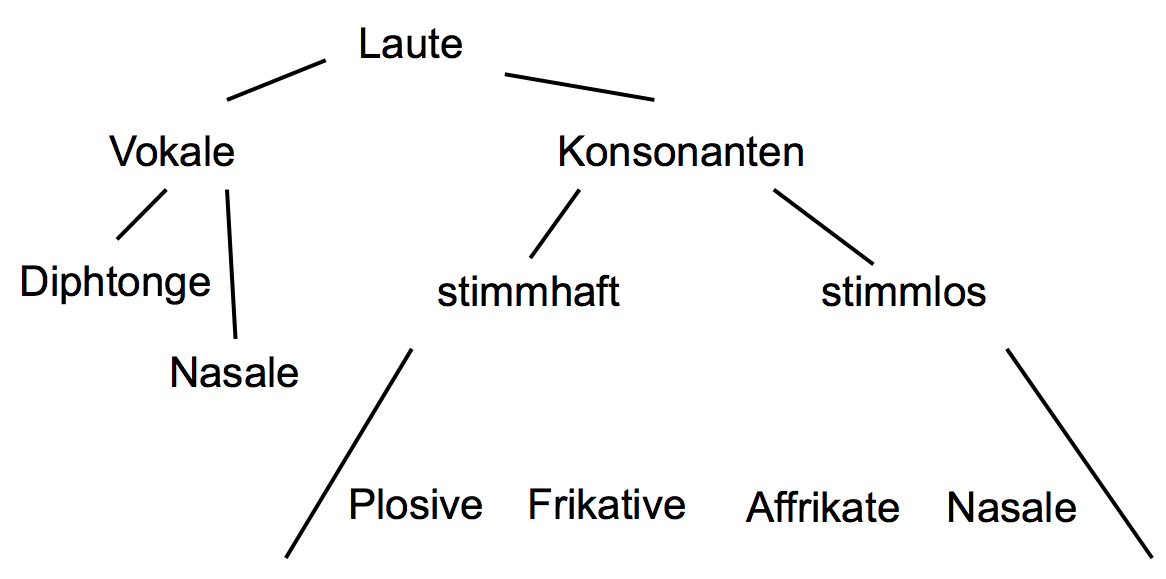
\includegraphics[width=0.75\textwidth]{phoneme_systematisch}
	\end{center}
\end{sectionbox}

\columnbreak

% SECTION: GRAMMATIKEN =================================================
\section{Grammatiken}
% ======================================================================
\begin{symbolbox}
	Natürlichsprachige Systeme; Modellierung von Dialogen. 
\end{symbolbox}

\begin{sectionbox}
	\subsection{Kontextfreie Grammatiken (CFG)}
	$ \mathcal G = \left\{ V, T, P, S \right\} $ mit 
	\begin{itemize}
		\item $V \equiv$ Variable (Großbuchstaben)
		\item $T \equiv$ Terminale (Kleinbuchstaben)
		\item $P \equiv$ Produktionsregel ($A \rightarrow \alpha $ mit $A \in \left\{V \right\}$ und $\alpha \in \left\{ V \cup T \right\} $)
		\item $S \equiv$ Startsymbol
	\end{itemize} 
	
	\subsubsection{Chomsky-NormalForm (CNF)}
	Enthält nur Produktionsregeln, bei denen auf der rechten Seite nur zwei Variablen oder nur ein terminaler Ausdruck steht: 
	\begin{emphbox}
		$A \rightarrow BC$ oder $A \rightarrow a$
	\end{emphbox}
	
	\subsubsection{Backus-Naur-Form (BNF)}
	Formal exakte Definition von Programmiersprachen. Nichtterminalsymbole werden syntaktische Variablen genannt und durch $<$ $>$ gekennzeichnet. Darstellung von Wiederholungen durch Rekursion. 
	\begin{itemize}
		\item $|$ Alternative
		\item $(\dots)$ Gruppierung
		\item $[\dots]$ oder $(\dots)?$ Option
		\item $(\dots)*$ optionale Wiederholung (keinmal, ein- oder mehrfach)
		\item $(\dots)+$ Wiederholung (ein- oder mehrfach)
	\end{itemize}
	
	\subsubsection{Erweiterte Backus-Naur-Form (EBNF)}
	\begin{itemize}
		\item $[\dots]$ Option
		\item ${\dots}$ optionale Wiederholung (keinmal, ein- oder mehrfach)
		\item $n*$ abgezählte Wiederholung
	\end{itemize}
	
	\subsubsection{Parsing}
	Satzgenerierung: Produktionsregeln solange anwenden, bis alle Variablen V durch terminale Symbole T ersetzt sind; Parse-Tree; Ambiguitäten; 
	
	\subsubsection{Anwendung von Grammatiken in KI}
	Sprache; Mustererkennung; 
\end{sectionbox}

\begin{sectionbox}
	\subsection{Beispiele Grammatiken}
	Palindrom-String:
	\begin{equation*}
	S \rightarrow aSa | bSb | a* | b*
	\end{equation*}

	Doppelte Anzahl a wie b:
	\begin{equation*}
	\begin{split}
		& S \rightarrow A | SA | AS | aSC | CSa | aSD | DSa | bSB | BSb \\
		& A \rightarrow Bb | Ca | Da \\
		& B \rightarrow aa \quad C \rightarrow ab \quad D \rightarrow ba \\
	\end{split}
	\end{equation*}

	Grammatik-Grammatik:\\
	S (Satz), NP (Nominalphrase), VP (Verbalphrase), PP (Päpositionalphrase), DET (Determinator, Artikel), ADJ (Adjektiv), AUX (Hilfswort), V (Verb), PRE (Präposition) und N (Nomen)
	\begin{equation*}
	\begin{split}
		&  \text{S} \ra \text{NP VP} | \text{VP NP}\\
		& \text{NP} \ra  \text{DET N} |  \text{ADJ N} |  \text{DET NP} |  \text{NP PP}\\
		&  \text{VP} \ra  \text{V NP} |  \text{AUX V} |  \text{V PP} |  \text{V NP} |  \text{VP PP} |  \text{AUX VP}\\
		&  \text{PP} \ra  \text{PRE NP}\\
		&  \text{DET} \ra  \text{"`der"', "`die"', "`das"',...}\\
		&  \text{ADJ} \ra  \text{"`klein"', "`groß"',...}\\
		&  \text{AUX} \ra  \text{"`wird"',...}\\
		&  \text{V} \ra  \text{"`streicheln"',...}\\
		&  \text{PRE} \ra  \text{"`in"', "`mit"',...}\\
		&  \text{N} \ra  \text{"`Junge"', "`Hund"', "`Hand"',...}\\
	\end{split}
	\end{equation*}
\end{sectionbox}

\columnbreak

% SECTION: AUTOMATENTHEORIE ============================================
\section{Automatentheorie}
% ======================================================================
\begin{symbolbox}
	Verarbeitung von Symbolfolgen; Modellierung von Dialogen; 
\end{symbolbox}

\begin{sectionbox}
	\subsection{Zustandsautomat}
	Graphenform; bestimmte Anzahl von Knoten (Zustände) und Verbindungen (Transitionen).
	\begin{equation*}
	Z = (\mathcal S, \mathcal X, \ma T, s_0, \mathcal F )
	\end{equation*}
	\begin{itemize}
		\item $\mathcal S$ Set mit endlicher Anzahl Zustände
		\item $\mathcal X$ zulässiges Alphabet für die zu verarbeitende Symbolfolge X
		\item $\ma T$ Transitionsfunktionen für die Zustände in $\mathcal S$
		\item $s_0$ Anfangszustand
		\item $\mathcal F$ ein Set von festgelegten Endzuständen
	\end{itemize}
	Transitionsfunktion als Regel: $t(s^−, x_i) = s^+$
	\begin{cookbox}{Umwandlung: Zustandsautomat in Grammatik}
		\item Zustänge werden Variable: $\mathcal S \Ra V$
		\item Eingabealph. wird zu Terminal: $\mathcal X \Ra T$
		\item Transitionen werden Produktionsregeln: $\ma T \Ra \P$,\\
		z.B. $P = \{S \ra aA, A ra bA $
		\item Für jeden Endzustand $s_E$ erstelle Produktionsregel,\\
		z.B. für B als Endzustand $\Ra P = \{\dots,B\ra \epsilon\}$
	\end{cookbox}
	\vspace{-1em}\paragraph{Beispiel für einen deterministischen Zustandsautomaten}\ \\
	\parbox{0.5\textwidth}{
		\begin{equation*}
			\begin{aligned}
				\mathcal S &= \{s_0,s_1,s_2,s_3\}\\
				\mathcal X &= \{0, 1\}\\
				\mathcal F &= \{s_0\}
			\end{aligned}
		\end{equation*}
	}
	\parbox{0.4\textwidth}{ 
		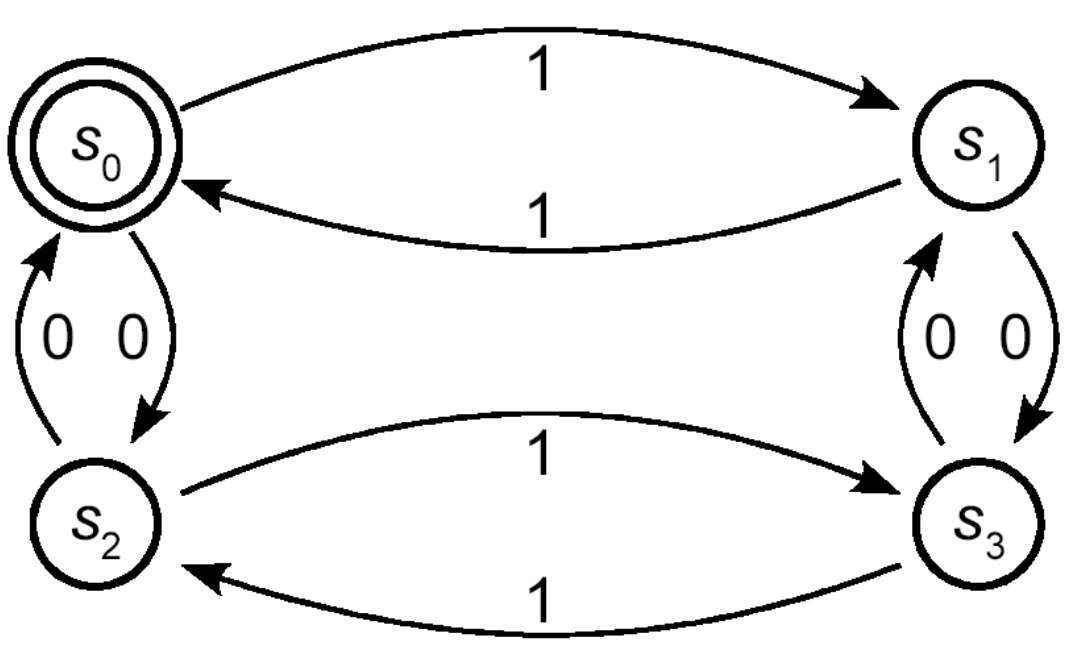
\includegraphics[width=0.3\textwidth]{zustandsautomat}
	}\\
	Transitionsregeln in Tabellenform: \\
	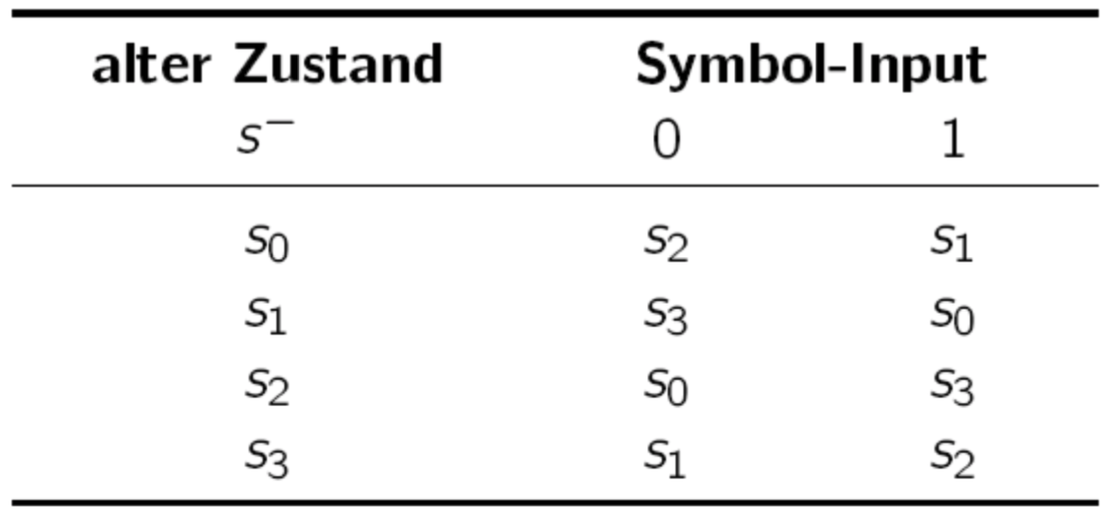
\includegraphics[width=0.4\textwidth]{transitionsregeln_tab}
	\vspace{-1em}\paragraph{Beispiel für einen nicht-deterministischen Zustandsautomaten}\ \\
	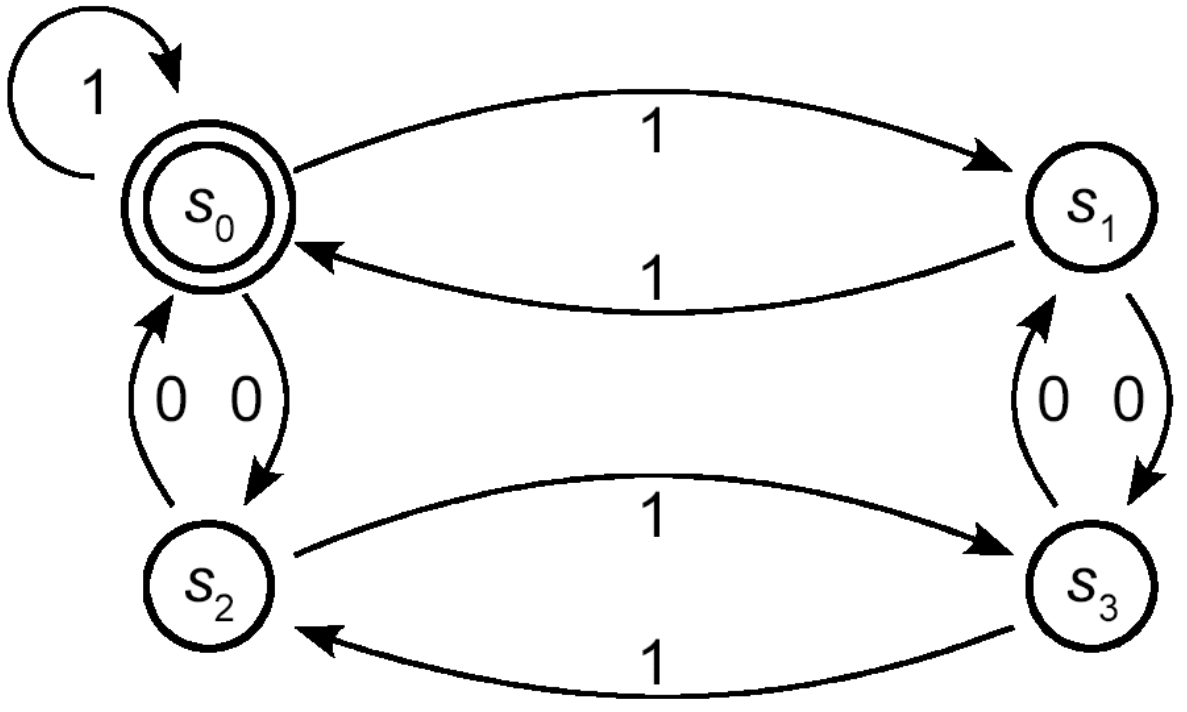
\includegraphics[width=0.3\textwidth]{zustandsautomat_nicht_det}
	
\end{sectionbox}

\begin{sectionbox}
	\subsection{Kellerautomaten}
	Komplexere Grammatiken; Erweiterung mit Stack (LIFO-Queue); Transition abhängig von Stack und Eingang; Stack leer $\Ra$ Folge akzeptiert; 
	\begin{equation*}
	Z = (\mathcal S, \mathcal X, \mathcal Y, \ma T, s_0, y_0 \mathcal F)
	\end{equation*}
	\begin{itemize}
		\item $\mathcal S$ Set mit endlicher Anzahl Zustände
		\item $\mathcal X$ zulässiges Alphabet für die zu verarbeitende Symbolfolge X
		\item $\mathcal Y$ zulässiges Alphabet für den Stack
		\item $\ma T$ Transitionsfunktionen für die Zustände in $\mathcal S$
		\item $s_0$ Anfangszustand
		\item $y_0$ Startsymbol für den Stack
		\item $\mathcal F$ ein Set von festgelegten Endzuständen (leer wenn Endzustand über leeren Stack definiert ist)
	\end{itemize}
	\vspace{-1em}\paragraph{Beispiel für einen Kellerautomaten:}\ \\
	\parbox{0.5\textwidth}{
		\begin{equation*}
		\begin{aligned}
			\mathcal S &= \{S_0,S_1\}\\
			\mathcal X &= \{a, b\}\\
			\mathcal Y &= \{\#, a\}\\
			y_0 &= \#\\
			\mathcal F &= \{\} \text{ (Ende durch leeren Stack)}
		\end{aligned}
		\end{equation*}
	}
	\parbox{0.5\textwidth}{ 
		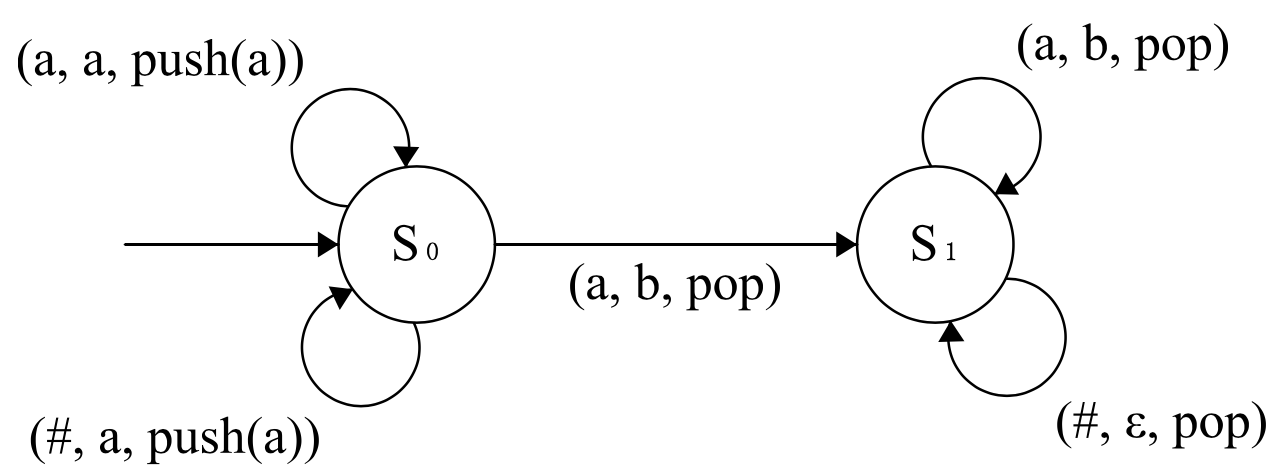
\includegraphics[width=0.5\textwidth]{kellerautomat}
	}\\
	Generiert Sprache: $L(a^nb^n)$ mit $n>0$
	\vspace{-1em}\paragraph{Angaben in Klammern:}\ \\
	(Voraussetzung auf Stack $\in \mathcal Y$, Eingabe $\in \mathcal X$, Aktion push($\dots$)/pop)
\end{sectionbox}

\columnbreak

% SECTION 3: SPRACHERKENNUNG ===========================================
\section{Spracherkennung}
% ======================================================================
\begin{symbolbox}
Spracherkennung beschäftigt sich mit der Untersuchung und Entwicklung von Verfahren, die Automaten, insbesondere Computern, die gesprochene Sprache der automatischen Datenerfassung zugänglich macht.
\end{symbolbox}

\begin{sectionbox}
	\subsection{Klassifizierung}
	Zuordnung zu Bedeutungseinheiten; Merkmalsextraktion; Merkmalsvektor; Merkmalsraum; Klassen; Training; 
\end{sectionbox}

\begin{sectionbox}
	\subsection{Abstandsklassifikatoren}
	Distanz eines Mustervektors zu Klasse;
	\begin{itemize}
		\item $\vec x$ unbekannter, zu klassifizierende Mustervektor
		\item $\vec r_{k,i}$ i-ter Referenzvektor für die k-te Klasse
		\item $\vec m_k$ Klassenzentrum der Klasse k
		\item $d_k(\vec x, \vec m_k)$ Abstandsformel
		\item $k_x$ Klasse mit minimalen Abstand zu $\vec x$
	\end{itemize} 
	Formeln
	\begin{equation*}
	\begin{aligned}
		\vec m_k &= \frac{1}{M_k} \sum\limits^{M_k}_{i=1} \vec r_{k,i} \\
		d_k (\vec x, \vec m_k) &= (\vec x - \vec m_k)^T \cdot \ma W_k \cdot (\vec x-\vec m_k) \\
		k_x &= \underset{x}{\mathrm{argmin}}\ d_k(\vec x, \vec m_k)
	\end{aligned}
	\end{equation*}
	
	Trennfunktion:
	\begin{equation*}
		d_1 (x, m_1) - d_2 (x, m_2) = 0
	\end{equation*}

	Gewichtsmatrix $W_k$ entscheidend über Ergebnis; $m_k$ wird im Training ermittelt; $x$ gehört zur Klasse k mit minimalen Abstand; 
	\vspace{-1em}\paragraph{Quadratischer Abstand} $W_k$ ist Einheitsmatrix; Trennfunktion ist eine Gerade;
	\vspace{-1em}\paragraph{Mahalanobis Abstand} Inverse der Kovarianzmatrix; Abhängig von Klasse; Bestandteil des Trainings; Trennfunktion ist Kegelschnitt (Gerade, Ellipse, Parabel, Hyperbel).

	\begin{equation*}
	\begin{split}
		& \ma W_{K,k} = \frac{1}{M_k} \sum\limits^{M_k}_{i=1} \vec r_{k,i} \cdot r^T_{k,i} \quad -m_k \cdot m_k^T \\
		& A^{-1} = \frac{1}{ad-bc}\begin{bmatrix} d & -b \\ -c & a \end{bmatrix}
	\end{split}
	\end{equation*}
\end{sectionbox}

\begin{sectionbox}
	\subsection{Cepstrum}
	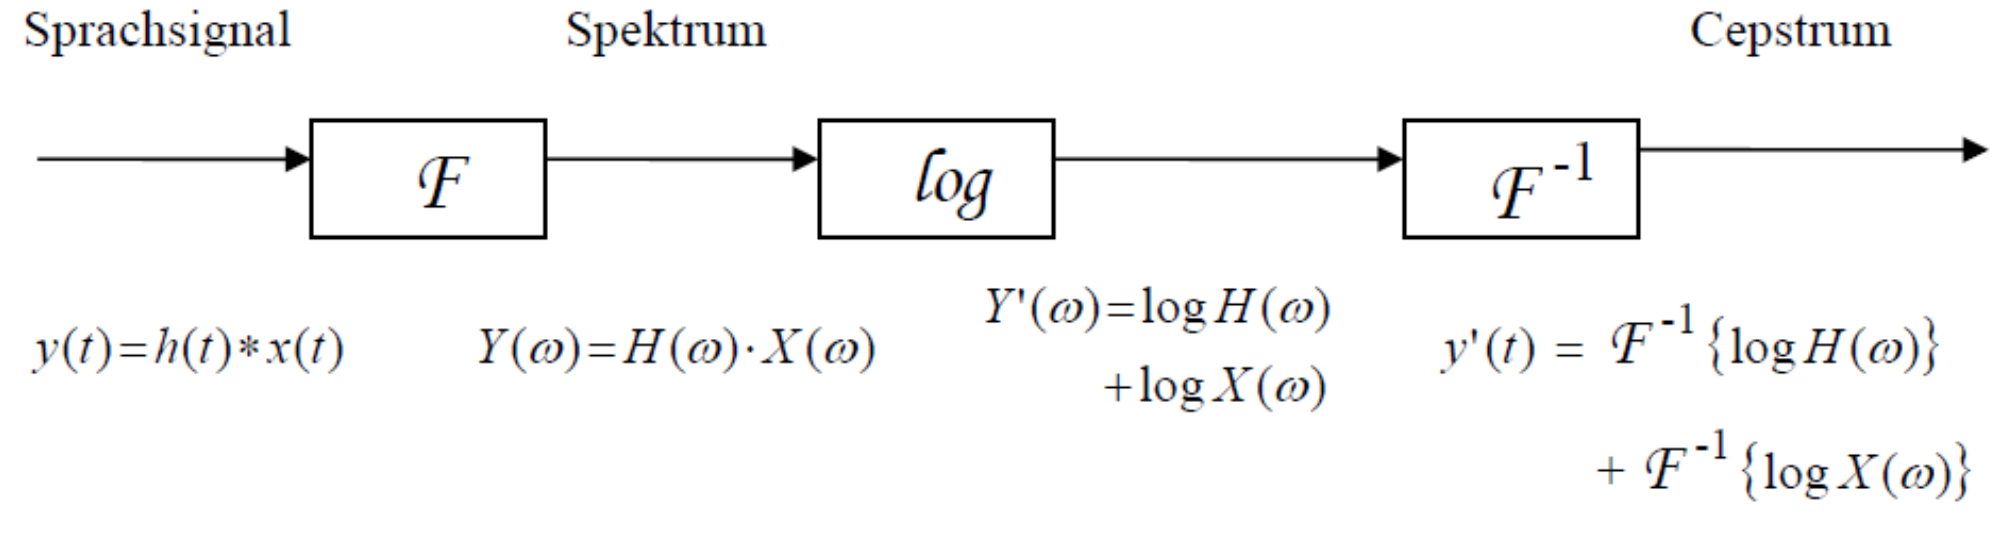
\includegraphics[width=\textwidth]{cepstrum}
	Praktische Berechnung:
	\begin{itemize}
		\item Selektion eines Zeitfensters für das betrachtete Sprachsignal
		\item Fourier-Transformation dieses Signals in den Frequenzbereich
		\item Bilden des Betrags des resultierenden (komplexen) Spektrums
		\item Logarithmierung des Amplitudenspektrums
		\item Rücktransformation mit inverser FT
	\end{itemize}
	
\end{sectionbox}

\columnbreak

% SECTION: HIDDEN-MARKOV-MODELLE =======================================
\section{Hidden-Markov-Modelle und Algorithmen}
% ======================================================================
\begin{symbolbox}Wahrscheinlichkeit
Statistischer Klassifikator. Liefert Wahscheinlichkeit $p$, dass eine Beobachtung einer bestimmten Klasse zugeordnet werden kann. Klassifizieren ganze Sequenzen (dynamische Folgen). "`Finde diejenige Klasse, die die Beobachtung $o=(o_1, o_2, \dots , o_t)$ am besten nachbilden kann."'.  
\end{symbolbox}

\begin{sectionbox}
	\subsection{Markov-Modelle (MM)}
	Abbildung stochastischer Prozesse, deren aktueller Zustand nur vom vorausgegangenen Zustand abhängt.
	\begin{itemize}
		\item Matrix der Übergangswkt.: $\ma A = p \left\{ q_{t+1} = s_j | q_t = s_i \right\}$
		\item Vektor der Einsprungswkt.: \\ $\vec e = (p(q_1 = s_1), \dots , p(q_1 = s_N))^T$
	\end{itemize}
	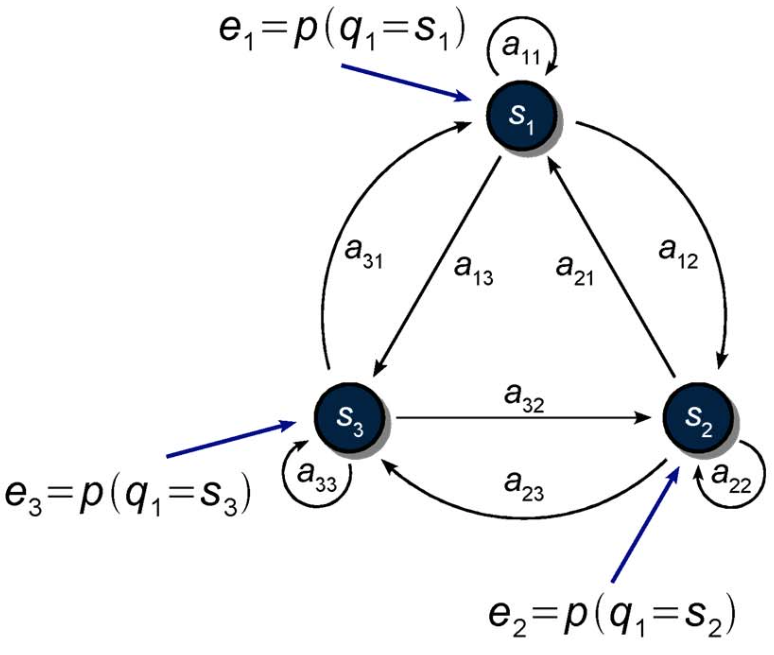
\includegraphics[width=0.8\textwidth]{mm}	
\end{sectionbox}

\begin{sectionbox}
	\subsection{Hidden-Markov-Modelle (HMM)}
	Stochastische Version eines endlichen Zustandautomaten; Zustandsübergänge und Symbolemissionen nicht deterministisch.
	\begin{itemize}
		\item Matrix $\ma A$ und Vektor $\vec e$ siehe MM
		\item Beobachtungsfolge: $\vec o = (o_1, \dots, o_T)^T$
		\item Alphabet: $\vec v = (v_1, \dots, v_M)^T$
		\item Beobachtungswahrscheinlichkeiten: $b_{mi}=p(v_m|s_i)$
		\item Matrix der Beobachtungswahrscheinlichkeiten: \\
		\begin{equation*}
			B = \begin{bmatrix}
				p(v_1 | s_1) & \dots & p(v_1 | s_N) \\
				\vdots & \ddots & \vdots \\
				p(v_M | s_1) & \dots & p(v_M | s_N) \\
		\end{bmatrix} \\ 
		\end{equation*}
	\end{itemize}
	Zusammengefasste Parameter des HMMs: $\lambda = (\vec e, \ma A, \ma B)$\\
	Beobachtungs- bzw. Produktionswkt.: $p(\vec o | \lambda )$ \\
	Dabei durchlaufene (vorborgene/hidden) Zustandsfolge: \\ $\vec q = (q_1, \dots, d_T)$

	\begin{tablebox}{p{\textwidth}}
	\emph{HMM - Eigenschaften} \\ % topicbox
	\cmrule
	\emph{Ergodisches HMM} \quad Es kann aus jedem Zustand in jeder andere Zustand erreicht werden; A ist voll besetzt \\
	\emph{Links-Rechts-HMM} \quad keine Rücksprünge; kausal; A hat rechte obere Dreiecksform; Graphisch nach rechts aufsteigend 
	\end{tablebox}
	
	\subsubsection{Klassifizierung mit HMM}
	Pro Klasse ein HMM; das HMM welches die größte Produktionswahrscheinlichkeit $p(o|\lambda_k)$ liefert, repräsentiert die gesuchte Klasse $k_x$;
	 
	\subsubsection{Training von HMM}
	Kompensation von Störungen; Bed.: geeignete Parameter $\lambda_k$; Training mit iterativen Verfahren; $\Ra$ Baum-Welch-Algorithmus
\end{sectionbox}

\columnbreak

\begin{sectionbox}
	\subsection{HMM in der Spracherkennung}
	\begin{symbolbox}
	Cepstrum;  Merkmalsexrahierung; 12D Merkmalsvektor;
	\end{symbolbox}

	\subsubsection{Modelle}
	Einzelworterkenner vs. fließende Sprache; Phoneme, kleinste bedeutungsunterscheidenden Lauteinheiten; HMM pro Phonem; Pausen; 

	\subsubsection{Training}
	Zusammenfassung der Phonem HMM zu einem HMM; 

	\subsubsection{Erkennung}
	Wörterbücher, Grammatiken, Wahrscheinlichkeiten bestimmter Phonemkombinationen, Sprachmodelle für Wortkombinationen; 
\end{sectionbox}

\begin{sectionbox}
	\subsection{HMM-Algorithmen}
	
	\subsubsection{Trellis}
	Mathematische Formel zur Berechnung der Beobachtungswkt.\\ 
	Für verschiedene Wege $q$ gilt: \\ 
	$p(\vec o, \vec q | \lambda_k) = e_{q1} b_{q1} (o_1) \prod\limits^T _{t=2} a_{q_{t-1} q_t} b_{q_t} (o_t)$
	Beobachtungswahscheinlichkeit:
	\begin{equation*}
	\begin{aligned}
		p(\vec o | \lambda_k) &= \sum\limits_{q \in Q} p(\vec o, \vec q | \lambda_k) \\
		&= \sum\limits_{q \in Q} e_{q1} b_{q1} (o_1) \prod\limits^T _{t=2} a_{q_{t-1} q_t} b_{q_t} (o_t)
	\end{aligned}
	\end{equation*}
	Benötigte OPS $\sim 2T \cdot N^T$ (sehr rechenintensiv)\\
	
	\subsubsection{Vorwärts-Algorithmus}
	Vorwärts-Wahrscheinlichkeit:

	$\alpha_t (i) = \P(o_1, o_2, \dots , o_t , q_t = s_i | \lambda_k)$

	d.h. die Wahrscheinlichkeit, dass die Teilbeobachtung $o_i$ emittiert werden und das sich das HMM zu t im Zustand $s_i$ befindet; 

	\begin{cookbox}{Vorwärts-Algorithmus (Rekursiv)}
		\item Initialisierung: \\
			$\alpha_1(i) = e_i b_i (o_1), \quad 1 \leq i \leq N $\\
		\item Induktion: \\
			$ \alpha_{t+1} (j) = \left[ \sum\limits_{i=1}^N{\alpha_t (i) a_{ij}} \right] b_j (o_{t+1}) $\\
			$  \quad 1 \leq t \leq T-1; \quad 1 \leq j \leq N;$\\
		\item Terminierung \\
			$\P(o|\lambda_k )= \sum\limits_{i=1}^N \alpha _T (i)$\\
	\end{cookbox}
	Benötigte OPS $\sim T \cdot N^2$
\end{sectionbox}

\begin{sectionbox}
\subsubsection{Baum-Welch-Algorithmus}
Rückwärtswahrscheinlichkeit:

 $\beta_t(i) = P(o_{t+1}, o_{t+2}, \dots , o_{T} | q_t = s_i , \lambda _k)$; 

d.h. Wahrscheinlichkeit, die restlichen Teilbeob. zu emmttieren;

\begin{cookbox}{Baum-Welch-Algorithmus (Rekursiv)}
	\item Initialisierung\\
		 $\beta_T (i) = 1 \quad 1 \leq i \leq N $\\
	\item Induktion\\
		$\beta_t(i) = \sum\limits_{j=1}^N a_{ij} b_j (o_{t+1}) \beta_{t+1} (j)$\\
		$t = T-1, T-2, \dots 1 \quad 1 \leq i \leq N$\\
\end{cookbox}
 
Wahrscheinlichkeit, dass sich dass HMM zu t im Zustand $s_i$ befindet und o emmitiert wird; Summe drüber $\Ra$  "`alle Aufenthalte im Zustand $s_i$"'
\begin{equation*}
\gamma _t (i) = \frac{\alpha_t (i) \beta_t (i)}{\sum \limits_{i=1}^N \alpha_t (i) \beta_t (i)}
\end{equation*}

Wahrscheinlichkeit, dass sich das HMM zu t in $s_i$ und zu t+1 in $s_j$ befindet; Summe drüber $\Ra$ "`aller Übergänge von $s_i$ zu $s_j$; 
\begin{equation*}
\begin{split}
&\xi_t (i,j) = \frac{\alpha _t (i) a_{ij} b_j (o_{t+1}) \beta_{t+1}(j)}{\sum \limits_{i=1}^N \alpha_t (i) \beta_t (i)}\\
&\gamma_t (i) = \sum\limits_{j=1}^N \xi
\end{split}
\end{equation*}

\end{sectionbox}

\begin{sectionbox}
\subsubsection{Viterbi-Algo}
Berechnet die Beobachtungswahscheinlichkeit des wahrscheinlichsten Pfades.
\begin{cookbox}{Viterbi-Algorithmus}
	\item Initialisierung: \\
		$\delta_1 (i) = e_i b_i (o_1) \quad 1 \leq i \leq N $\\
		$\psi _1 (i) = 0$\\
	\item Induktion: \\
		$\delta_t (j) = \max\limits_{1 \leq i \leq N }\left[ \delta_{t-1} (i) a_{ij} \right] b_j (o_t)$\\
		$\psi_t(j) = \underset{1 \leq i \leq N}{\operatorname{argmax}} \left[\delta_{t-1}(i) a_{ij} \right]$\\
		$2 \leq t \leq T; \quad 1 \leq j \leq N$\\
	\item Terminierung: \\
		$P^* = \max\limits_{1 \leq i \leq N} [\delta_t(i)]$\\
		$q_T^* = \max\limits_{1 \leq i \leq N} [\delta_t(i)]$\\
	\item Ermittlung der wahrsch. Zustandsfolge:\\
		$q_t^* = \psi_{t+1}(q^*_{t+1})$\\
		$t= T-1, T-2, \dots , 1$\\
\end{cookbox}
\end{sectionbox}

\columnbreak

% SECTION 4: GRUNDLAGEN INTELLIGENTER SYSTEME ==========================
% \section{Grundlagen intelligenter Systeme}
% ======================================================================

% SECTION: SUCHVERFAHREN ===============================================
\section{Suchverfahren}
% ======================================================================
\begin{symbolbox}
	Formulierung und Darstellung eines Problems im Zustandsraum; Graphen-Darstellung; Suchbaum;
\end{symbolbox}

\begin{emphbox}
	Zyklische Wiederholungen unterbinden (gerichtete Kanten im Baum).
\end{emphbox}

\begin{sectionbox}
	\subsection{Allgemeiner Algorithmus für Suche}
	\begin{cookbox}{Suchalgorithmus}
		\item Initialisiere Queue
		\item Schreibe Startknoten in \textcolor{orange}{Queue}
		\item Wiederhole:
		\begin{enumerate}
			\item Queue leer? $\Ra$ "Ziel nicht gefunden"
			\item Entnehme nächsten Knoten
			\item Knoten == Ziel? $\Ra$ "Ziel erreicht"
			\item Schreibe alle Kinder des Knotens in die Queue
			\item \textcolor{orange}{Update Queue}
		\end{enumerate}
	\end{cookbox}
	Art des Algorithmus betimmt die Art der \textcolor{orange}{Queue}, und damit die Update-Funktion:
	\begin{tablebox}{ll}
		\emph{Suchalgorithmus} & \emph{Art der Queue} \\ \cmrule
		Breitensuche &  FIFO-Queue \\
		Tiefensuche & LIFO-Queue (Stack) \\
		A-Suche & Priotiy-Queue \\
		A*-Suche & Priotiy-Queue mit heuristischen Kosten als Priorität  \\
		Dijkstra & Priotiy-Queue mit bisherige Weg als Heuristik \\
	\end{tablebox}
\end{sectionbox}

\begin{sectionbox}
\subsection{\textcolor{darkgreen}{Tiefensuche} und \textcolor{red}{Breitensuche}}
\begin{enumerate}
	\item einelementige Liste mit Wurzelknoten
	\item bis Liste leer / Ziel erreicht: \\ -prüfe erstes Element auf Zielknoten \textcolor{darkgreen}{bzw. max. Suchtiefe} \\-wenn ja, fertig \\ - wenn nein, entferne dieses Element und füge all seine Nachfolger \textcolor{darkgreen}{ an gleicher Stelle} / \textcolor{red}{am Ende} ein.
\end{enumerate}

Vorraussetzung: Elemente der Warteliste werden systematisch erzeugt; Suchtiefe wird geeignet groß festgesetzt / ausgewertete Suchbaum muss gespeichert werden; 
\end{sectionbox}

\begin{sectionbox}
\subsection{Heuristische Suche / A-Algorithmus}
Verarbeitung zusätzlicher Informationen; Bewertungsmöglichkeit für Erfolgsaussichten eines bestimmten Pfades; Entscheidungen ordnen; Vielversprechende Alternative zuerst, "`dem atm billigsten folgen"'; Heuristik besteht in Definition einer geeigneten Bewertungs (Kostenfunktion) $f(n)$:
\begin{equation*}
f(n) = g(n) + h(n)
\end{equation*}
Bewertungsfunktion = Bisherige Kosten + Schätzfunktion (hier: falsche Plättchen)

Falls $h(n) \equiv 0$ gewählt wird identisch zur Breitensuche
\end{sectionbox}

\begin{sectionbox}
\subsection{A*-Algorithmus}
Schätzfunktion $h(n)$ monoton, d.h. Kosten werden nicht überschätzt; terminiert wenn Zielknoten gefunden und keine geringere Kostenschätzung existiert; A* somit optimaler Pfad; wird die optimale Kostenfkt $h1^*(n)$ verwendet, so wird kürzester Pfad auf Anhieb gefunden (sprich: informierte Suche); Liste mit allen Elementen erstellen + sortieren; dem insg. billigsten folgen; nix verwerfen.
\end{sectionbox}

\columnbreak

\section{Logik und Theorembeweisen}
\begin{symbolbox}
Wissen algorithmisch darstellen; Fakten ableiten; Behauptungen bestätigen / widerlegen; 
\end{symbolbox}

\begin{sectionbox}
\subsection{Aussagenlogik}
atomare Aussagen; wahr oder falsch; UND , ODER, NICHT; Implikation $\Rightarrow$; 
\end{sectionbox}

\begin{sectionbox}
\subsection{Prädikatenlogik}
Analyse und Bewertung von Beziehungen und logischen Verknüpfungen\\
1. Ordnung $\Ra$ nur Veränderung von Objekten, nicht Prädikaten\\
Prädikate und Funktionen, Konstanten, Variablen, Funktionen, Negation, Disjunktion, Konjunktion, Existenz-Quantor, All-Quantor, Implikation, Äquivalenz.\\\\
Beispiel: "`In jeder Stadt gibt es einen Bürgermeister"' \\
$(\forall x) \left\{ \text{Stadt}(x)  \Rightarrow (\exists y) \left[ \text{Mensch}(y) \cdot \text{Bgm}(x,y) \right] \right\}$\\\\
Regeln und Zusammenhänge aufstellen; $\Ra$ Regelwerk (Axiome); Frage (Theorem); Beweis durch Wahrheitstabelle oder Umformen der Regeln und Schlussfolgern (Resolution, Unifikation - effektiver); 
\end{sectionbox}

\begin{emphbox}
\emph{Umformregeln:}
\begin{enumerate}
	\item Doppelte Negation $\neg \neg A \equiv A$
	\item Idempotenz $ A + A \equiv A$ und $ A \cdot A \equiv A$
	\item Kommutativität $A + B \equiv B + A$
	\item Assoziativität $A + (B + C) \equiv (A + B) + C$
	\item Distributivität $A + (B \cdot C) \equiv (A + B) \cdot (A + C)$
	\item De Morgan $\neg(A \cdot B) \equiv \neg A + \neg B$
	\item Kontrapositiv $A \Rightarrow B \equiv \neg B \Rightarrow \neg A$ 
	\item $ A \Rightarrow B \equiv \neg A + B$ 
	\item $ A \Leftrightarrow B \equiv (A \Rightarrow B ) \cdot (B \Ra A) \equiv (A \cdot B) + (\neg A \cdot \neg B) $
	\item $ \neg (\forall x)A(x) \equiv (\exists x)(\neg A(x))$ 
	\item $ \neg (\exists x) A(x) \equiv (\forall x) (\neg{}A(x)) $ 
	\item $ (\forall x)(A(x) \cdot B(x)) \equiv (\forall x)A(x) \cdot (\forall y )B(y)$ 
	\item $ (\exists x)(A(x) + B(x)) \equiv (\exists x)A(x) + (\exists y)B(y)$
\end{enumerate}
\end{emphbox}

\begin{sectionbox}
\subsection{Standardformen}
Konjunktive Normalform (KNF): $(A_1 + A_2 + \dots) \cdot (B_1 + B_2 + \dots) \cdot \dots$ \\
Disjunktive Normalform: $(A_1 \cdot A_2 \cdot \dots) + (B_1 \cdot B_2 \cdot \dots) + \dots$
\begin{cookbox}{Regeln zur Umformung in Normalform:}
%\begin{enumerate}
	\item Eliminierung aller Äquivalenzen (\# 9)
	\item Eliminierung aller Implikationen (\# 8)
	\item Einziehung der Negation nach innen (\#6, \#10, \#11)
	\item Einführung neuer Variabeln für jeden Quantifizierer
	\item Eliminierung aller Existenz Quantoren
	\item Ausklammern der All-Quantoren und Entfallen dieser
	\item Anwendung des Distributivgesetzes zur Transformation in Konjunktive Normalform (\#5)
	\item Eliminierung der UND-Verknüpfungen durch Auflistung der Klauseln
	\item Einführung getrennter Variablen für jede Klausel
%\end{enumerate}
\end{cookbox}
\end{sectionbox}

\begin{sectionbox}
\subsection{Theorembeweis mit Resolutionsverfahren}
Allgemeines Resolutionsgesetz:\\
\begin{equation*}
	(X + A) \cdot (\neg X + B) \equiv (X + A) \cdot (\neg X + B) \cdot \underbrace{(A + B)}_{\text{Resolvente}}
\end{equation*}
Spezielles Resolutionsgesetz:
\begin{equation*}
	(X + A) \cdot (\neg X + A) \equiv A
\end{equation*}
Absorptionsgesetz:
\begin{equation*}
	(A + B) \cdot A \equiv A
\end{equation*}
Weitere Sonderfälle:
\begin{equation*}
\begin{aligned}
1.\ & A \\
& A \Ra B \equiv \neg A + B & R \equiv B \\
2.\ & A + B \\
& \neg A + B & R \equiv B + B = B \\
3.\ & A \\
& \neg A & R \equiv NIL \\
4.\ & A \Ra B \equiv \neg A + B \\
& B \Ra C \equiv \neg B + C & R \equiv \neg A + C \equiv A \Ra C\\
\end{aligned}
\end{equation*}

% Gegeben sind zwei Formel der Form: 
% 
% \begin{equation*}
% \begin{split}
% 	A_1 + A_2 + \dots + A_n + \textcolor{red}{ P } \\
% 	B_1 + B_2 + \dots + B_n + \textcolor{red}{ \neg P } \\
% 	\text{wird zu} \\
% 	A_1 + \dots  + A_n + B_1 + \dots +  B_n e\equiv R
% \end{split}
% \end{equation*}

Anwendung beim Theorembeweis: \\
Geg.: Set von $n$ existierenden und bewiesenen Axiomen $\mathcal S = \left\{S_1 \dots S_n \right\}$ ; Es gilt T zu beweisenn\\
Vorgehen: Erweiterung von $\mathcal S $ zu $\mathcal S^* = \left\{S_1 \dots S_n , \neg T \right\}$ Und Resolutionieren bis leere Klausel erzeugt wird. \\
Erklärung: Statt Beweis wird Unerfüllbarkeit seines Gegenteils gezeigt.

\begin{cookbox}{Tautologie beweisen: }
	\item Wahrheit auf KNF bringen
	\item Gegenteil auf KNF bringen
	\item Zeige, dass Gegenteil \{ \} ist. 
\end{cookbox}
\end{sectionbox}

\section{Wissensrepräsentation}
\begin{symbolbox}
	effizient speichern; strukturiert darstellen; Menge von Fakten, Regeln, Prozeduren, Modellen, Daten, Heuristiken; interpretierbar mit Hilfe von Repräsentationsmechanismen; 
\end{symbolbox}

\begin{sectionbox}
\subsection{Prädikatenlogik}
Aufteilung in Fakten und Regeln; Standardisiert durch KNF; Resolution als Inferenzmechanismus; Formulierung aufwändig und unnatürlich; zwingend Umformung in KNF;
\end{sectionbox}

\begin{sectionbox}
\subsection{Produktionsregeln}
keine Umformung in KNF; Wenn-Dann bleibt erhalten; Vorwärts- Rückwärtsverkettung als Inferenzmechanismus; Darstellung im UND/ODER-Graphen; Fakten als Blatt, Regeln als Verzweigung;

% TODO: Check if needed:
% \begin{cookbox}{Vorwärtsverkettung}
% 	\item Gültige Fakten einkreisen
% 	\item Suchen nach Regeln, in denen diese Fakten im Bedingungsteil der Regeln vorkommen
% 	\item Überprüfen ob Aktionsteil der Regeln eingeleitet werden kann
% 	\item Back to \#2
% 	\item Wenn keine neuen Regeln mehr feuern, überprüfen ob ein Ziel erfüllt wurde
% \end{cookbox}
% 
% \begin{cookbox}{Rückwärtsverkettung}
% 	\item Vorgabe eines möglichen Ziels
% 	\item Untersuchen der Bedingungen die zum erreichen dieses Ziels erfüllt sein müssen
% 	\item Formulierung dieser Bedingungen als neue Teilziele, back to \# 2
% 	\item Falls Ziel wg. Bedingungen nicht erreicht werden kann, back to \#1 mit anderem Ziel
% 	\item Wurden für ein Ziel alle Bedingungen erfüllt $\Ra$ Finish
% \end{cookbox}
\end{sectionbox}

\begin{sectionbox}
\subsection{Semantische Netze}
Graphische Modelle zur Darstellung von Wissen über beziehungen zw. Objekten; entsprechen etwa Fakten der Prädikatenlogik; Knoten = Objekte; Kanten = Prädikate; Verwendung bei natürlichssprachigen Systemen; keine 2 Knoten gleicher Beschriftung; Richtung der Kanten von Bedeutung; 
\end{sectionbox}

\begin{sectionbox}
\subsection{Rahmen}
Darstellung der Zerlegung von Objekten oder Situationen in ihre Bestandteile; Ähnlichkeit zu semantischen Netzen, wesentlich mächtiger und flexibler; FrameName - zentraler Knoten, Slots - Kanten, Filler - Knoten; \\
1. Suchverfahren zur Ermittlung von Beziehungen; \\
2. "`Rahmen-Abgleich"'; Fakten als Fragezeichen markiert; mit aktuellen Daten auffüllen; 
\end{sectionbox}

% SECTION 5: HANDSCHRIFTERKENNUNG ======================================
\section{Handschrifterkennung}
% ======================================================================

\begin{sectionbox}
	\subsection{Vorverarbeitung}
		\begin{cookbox}{Eingabemethoden}
			\item freie Eingabe (hohe Vorverarbeitung)
			\item liniengeführte Eingabe
			\item feldgeführte Eingabe
		\end{cookbox}
	Eingangssignal: $\vec x(t) = (x(t), y(t), p(t))^T$\\
	\begin{tablebox}{ll}
		x(t) & x-Koordinate\\
		y(t) & y-Koordinate\\
		p(t) & Druck (des Stifts)\\
	\end{tablebox}
\end{sectionbox}

\begin{sectionbox}
	\subsubsection{Abtastung}
		\begin{cookbox}{Abtastung / Neuabtastung}
			\item Diskretisierung von $\vec x(t)$ mit $n \cdot \Delta T \Ra $ zeitäquidistante Abtastung
			\item Lineare Interpolation der Stifttrajektorie
			\item Neuabtastung $\Ra$ ortsäquidistante Abtastpunkte $\vec x_{re}[k]$
		\end{cookbox}

		Länge einer Kurve $\vec r(t) = (x(t),y(t))^T$:\\ 
		$L(a,b) = \int \limits_a^b \sqrt{(\frac{\diff x(t)}{\diff t})^2 + (\frac{\diff y(t)}{\diff t})^2} \diff t$\\
		
		Druckkomponente: $p_n = p_1 + k\cdot(p_2 - p_1)$
\end{sectionbox}

\begin{sectionbox}
	\subsubsection{Korrekturen}
		\begin{cookbox}{Zeilenneigung (skew)}
			\item Horizontale Ausrichtung der Kernlinie des Geschriebenen
			\item Drehung um den Mittelpunkt $\vec m$ d. Kernlinie um den Winkel $\alpha_0$
			\item Bestimmung von $\alpha_0$ mit Projektionsprofilen oder Richtungshistogrammen in y-Richtung, $H_y(\alpha)$ muss möglichst klein sein
		\end{cookbox}

		Entropie: (B: Anzahl d. Bins, N($B_i$): Anzahl d. Punkte in Bin i)\\
		$H_y(\alpha) = \sum\limits_{i=1}^{B}I(i)$\\
		$I(B_i) = - \frac{N(B_i)}{\sum\limits_{j=1}^{B} N(B_j)} \text(ld) \frac{N(B_i)}{\sum\limits_{j=1}^{B} N(B_j)}$\\
		Regressionsgerade $y = mx+b$:\\
		$m=\frac{\sum \limits_{i=1}^{N}[(x_i - \ol x) (y_i - \ol y)]}{\sum \limits_{i=1}^{N} (x_i - \ol x)^2}$ und $b= \ol y - m \ol x$\\
		Rotation:\\
		$\vec x_{skew}[k] = \mat{ \cos \alpha_0 & -\sin \alpha_0 & 0 \\ \sin \alpha_0 & \cos \alpha_0 & 0 \\ 0&0&1} (\vec x_{re}[k] - \vec m)+ \vec m$\\
		

		\begin{cookbox}{Schriftneigung (slant)}
			\item Scherung der Schrift an der Grundlinie $y_S$
			\item Scherung um den Winkel $\phi_0$
			\item Bestimmun von  $\phi_0$ mit  Projektionsprofilen oder Richtungshistogrammen in x-Richtung, $H_x(\phi)$ muss möglichst klein sein
		\end{cookbox}

		Scherung:\\
		$\vec x_{slant}[k] = \mat{ 1 & -\tan\phi_0 & 0 \\ 0& 1 & 0\\ 0 & 0 & 1} (\vec x_{skew}[k]- \mat{0 \\ y_S \\ 0})+ \mat{0 \\ y_S \\ 0}$ \\
\end{sectionbox}

\begin{sectionbox}
			\begin{cookbox}{Schriftgröße}
				\item Schätzen der Referenzlinien
				\item Berechnung der Kernhöhe
				\item Normirung des Schriftzuges
			\end{cookbox}
			
			W: Höhe der Bins, P: Projektionsprofil\\
			Oberlängenlinie: $y_{ober} = y_{max}$, Unterlängenlinie: $y_{unter} = y_{min}$\\
			Kernlinie: $y_{kern}  = \text{argmin}(\frac{\diff}{\diff j}P_y(j))-0.5)W+ y_{min}$\\
			Basislinie: $y_{grund} = \text{argmax}(\frac{\diff}{\diff j}P_y(j))-0.5)W+ y_{min}$\\
			Kernhöhe: $h_{kern} = |y_{kern}-y_{grund}|$\\
			Normierung:\\
			$\vec x_{norm}[k] = \frac{1}{h_{kern}} \mat{x[k] - x_{min} \\ y[k] - (y_{grund} + \frac{h_{kern}}{2})}$
			
\end{sectionbox}

\begin{sectionbox}
	\subsection{Merkmalsextraktion}
		Extraktion aus dem normalisierten Schriftzug\\
		Sekantensteigungswinkel:\\
		$\theta[k] = \frac{\pi}{2} + \begin{cases}\arctan(\frac{\Delta y}{\Delta x}) - \frac{\pi}{2} \sgn(\Delta x) & \text{für } \Delta x \neq 0\\
								     \frac{\pi}{2} (1- \sgn(\Delta x) ) & \text{für } \Delta x = 0 \end{cases}$\\
$\Delta x = x_{norm}[k+1]-x_{norm}[k]$, $\Delta y = y_{norm}[k+1]-y_{norm}[k]$\\
		Richtungsänderung:\\
		$\Delta \theta[k] = \theta[k+1]-\theta[k]$\\
		5-dim. Merkmalsvektor:
		$\vec m[k] = \mat{\sin(\theta[k]) \\ \cos(\theta[k]) \\ \sin(\Delta \theta[k]) \\ \cos(\Delta \theta[k]) \\ p[k]}$
		
\end{sectionbox}

\begin{sectionbox}
	\subsection{Erkennung}
		Trainig und Erkennung läuft über Hidden-Markov-Modelle (HMM) mit Graphemen (z.B. Buchstabe, Sonderzeichen od. Ziffern) als kleinste Einheit\\
		Training: Baum-Welch-Alogrithmus\\
		Erkennung: Viterbi-Algorithmus\\
\end{sectionbox}


%%%%%%%%%%%%%%%%%%%%%%%%%%%%%%%%%%%%%%%%%%%%%%%%%%%%%%%%%%%%%%%%

\section{Dialogsystem (Anhang)}
\begin{symbolbox}
\begin{itemize}
	\item fortgeschrittene intuitive Ein-/Ausgabetechniken 
	\item Hohes Maß an Interaktivität durch Benutzerfreundlichkeit und ausgeprägte Dialogfähigkeit
	\item Intelligentes Systemverhalten, selbstständig logische Schlüsse ziehen; 
\end{itemize}
\end{symbolbox}
Teilgebiete der KI: Maschinelles Lernen, Bildverstehende Systeme, Expertensysteme, Robotik, Logik und automatisches Beweisen, natürlichsprachliche Systeme; 



% Dokumentende
% ======================================================================
\end{document}
